\documentclass[ucs,11pt]{beamer}

\usepackage[utf8]{inputenc}
\usepackage[english]{babel}
\usepackage{graphicx}


% Bla bla bla
% Das Template hab ich ein bisschen anpassen muessen, da pgfdeclareimage usw. irgendwie
% nicht mehr funktionieren wollte. Moeglicherweise aufgrund einer neuen Version o.Ae.
% So gehts aber auch.


% Template for talks using the Corporate Design of the Freie Universitaet
%   Berlin, created following the guidelines on www.fu-berlin.de/cd by
%   Tobias G. Pfeiffer, <tobias.pfeiffer@math.fu-berlin.de>
% This file can be redistributed and/or modified in any way you like.
%   If you feel you have done significant improvements to this template,
%   please consider providing your modified version to
%   https://www.mi.fu-berlin.de/w/Mi/BeamerTemplateCorporateDesign

% NOTE: Removed pgf because it didn't work for me.

%%% FU logo
% small version for upper right corner of normal pages
%\pgfdeclareimage[height=0.9cm]{university-logo}{FULogo_RGB}
%\logo{\pgfuseimage{university-logo}}
% large version for upper right corner of title page
%\pgfdeclareimage[height=1.085cm]{big-university-logo}{FULogo_RGB}
%\newcommand{\titleimage}[1]{\pgfdeclareimage[height=2.92cm]{title-image}{#1}}
%\titlegraphic{\pgfuseimage{title-image}}
%%% end FU logo

\logo{
\includegraphics[height=0.9cm]{FULogo_RGB.png}}
\newcommand{\titleimage}[1]{\titlegraphic{\includegraphics[height=2.92cm]{#1}}}

% NOTE: 1cm = 0.393 in = 28.346 pt;    1 pt = 1/72 in = 0.0352 cm
\setbeamersize{text margin right=2.5mm, text margin left=7.5mm}  % text margin

% colors to be used
\definecolor{text-grey}{rgb}{0.45, 0.45, 0.45} % grey text on white background
\definecolor{bg-grey}{rgb}{0.66, 0.65, 0.60} % grey background (for white text)
\definecolor{fu-blue}{RGB}{0, 51, 102} % blue text
\definecolor{fu-green}{RGB}{153, 204, 0} % green text
\definecolor{fu-red}{RGB}{204, 0, 0} % red text (used by \alert)

% switch off the sidebars
% TODO: loading \useoutertheme{sidebar} (which is maybe wanted) also inserts
%   a sidebar on title page (unwanted), also indents the page title (unwanted?),
%   and duplicates the navigation symbols (unwanted)
\setbeamersize{sidebar width left=0cm, sidebar width right=0mm}
\setbeamertemplate{sidebar right}{}
\setbeamertemplate{sidebar left}{}
%    XOR
% \useoutertheme{sidebar}

% frame title
% is truncated before logo and splits on two lines
% if neccessary (or manually using \\)
\setbeamertemplate{frametitle}{%
    \vskip-30pt \color{text-grey}\large%
    \begin{minipage}[b][23pt]{80.5mm}%
    \flushleft\insertframetitle%
    \end{minipage}%
}

%%% title page
% TODO: get rid of the navigation symbols on the title page.
%   actually, \frame[plain] *should* remove them...
\setbeamertemplate{title page}{
% upper right: FU logo
\vskip2pt\hfill
\includegraphics[height=1.085cm]{FULogo_RGB} \\
\vskip6pt\hskip3pt
% title image of the presentation
\begin{minipage}{11.6cm}
\hspace{-1mm}\inserttitlegraphic
\end{minipage}

% set the title and the author
\vskip14pt
\parbox[top][1.35cm][c]{11cm}{\color{text-grey}\inserttitle \\ \small \insertsubtitle}
\vskip11pt
\parbox[top][1.35cm][c]{11cm}{ \insertinstitute \\[3mm] \insertdate}
}
%%% end title page

%%% colors
\usecolortheme{lily}
\setbeamercolor*{normal text}{fg=black,bg=white}
\setbeamercolor*{alerted text}{fg=fu-red}
\setbeamercolor*{example text}{fg=fu-green}
\setbeamercolor*{structure}{fg=fu-blue}

\setbeamercolor*{block title}{fg=white,bg=black!50}
\setbeamercolor*{block title alerted}{fg=white,bg=black!50}
\setbeamercolor*{block title example}{fg=white,bg=black!50}

\setbeamercolor*{block body}{bg=black!10}
\setbeamercolor*{block body alerted}{bg=black!10}
\setbeamercolor*{block body example}{bg=black!10}

\setbeamercolor{bibliography entry author}{fg=fu-blue}
% TODO: this doesn't work at all:
\setbeamercolor{bibliography entry journal}{fg=text-grey}

\setbeamercolor{item}{fg=fu-blue}
\setbeamercolor{navigation symbols}{fg=text-grey,bg=bg-grey}
%%% end colors

%%% headline
\setbeamertemplate{headline}{
\vskip4pt\hfill\insertlogo\hspace{3.5mm} % logo on the right

\vskip6pt\color{fu-blue}\rule{\textwidth}{0.4pt} % horizontal line
}
%%% end headline

%%% footline
\newcommand{\footlinetext}{\insertshortinstitute, \insertshorttitle, \insertshortdate}
\setbeamertemplate{footline}{
\vskip5pt\color{fu-blue}\rule{\textwidth}{0.4pt}\\ % horizontal line
\vskip2pt
\makebox[123mm]{\hspace{7.5mm}
\color{fu-blue}\footlinetext
\hfill \raisebox{-1pt}{\usebeamertemplate***{navigation symbols}}
\hfill \insertframenumber}
\vskip4pt
}
%%% end footline


\titleimage{polygons}

\title[Zufällige Polygone]{Zufällige Polygone}
\subtitle{Projektvorstellung}
\institute[FU Berlin]{Freie Universität Berlin}
\date[08.11.2011]{8. November 2011}

\begin{document}

\begin{frame}[plain]
	\titlepage
\end{frame}

\begin{frame}{Goals}
	\begin{itemize}
	\item Testing framework for algorithms related to random polygons
	\item Step 1: Generate random polygons (fair, representative)
	\item Step 2: Run shortest path algorithm on polygon
	\item Step 3: Statistical analysis
	\end{itemize}
\end{frame}

\begin{frame}{Organisation}
  \begin{itemize}
    \item mailing list, git, redmine
    \item weekly meeting, protocol
    \item custom software process
      \begin{itemize}
        \item determine tasks, groups
        \item in groups: explain algorithms, implement
        \item presentation of results
        \item revison of tasks
        \item profit
      \end{itemize}
    \item java, elcipse, coding style
  \end{itemize}
\end{frame}

\begin{frame}{Architecture}
  \begin{center}
	  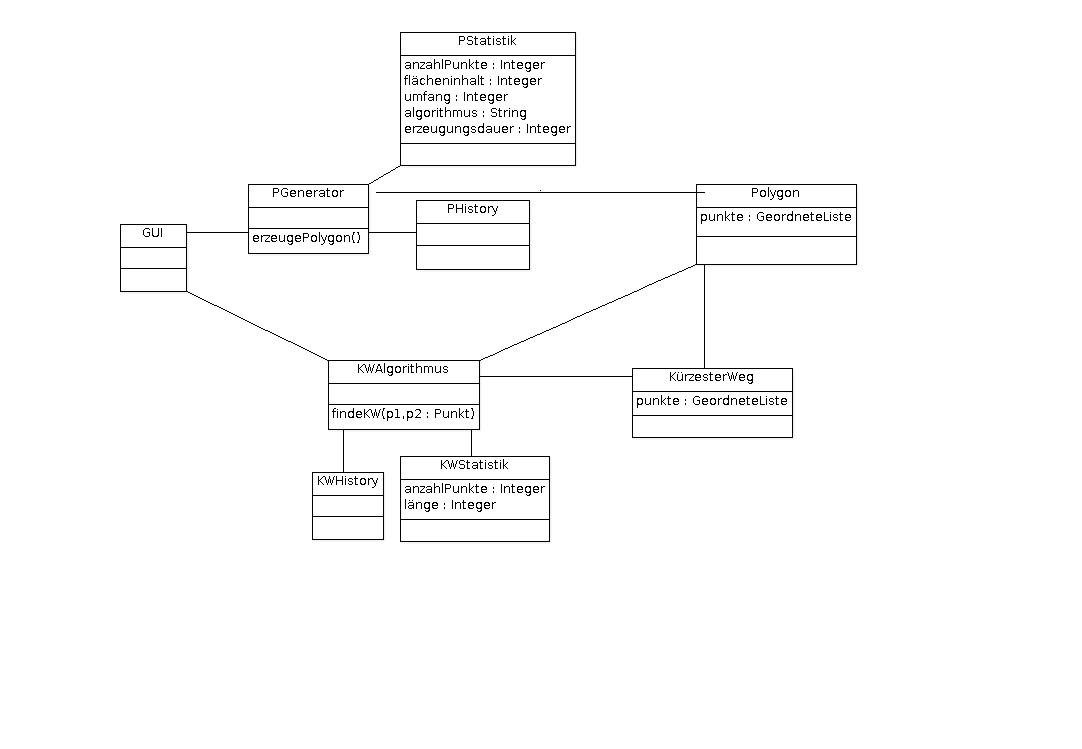
\includegraphics[width=\textwidth]{ClassDiagram.png}
  \end{center}
\end{frame}

\begin{frame}{Roadmap}
  \begin{itemize}
    \item until now
      \begin{itemize}
        \item interface polygon generator
        \item data structures scratch (except history objects)
        \item GUI scratch
      \end{itemize}
      \item next week
      \begin{itemize}
        \item first polygon algorithm
        \item interface shortest path generator
        \item data structures (except history objects)
      \end{itemize}
      \item before next presentation (mid december)
        \begin{itemize}
          \item all polygon algotithms
          \item shortest path generator
          \item GUI basic version
        \end{itemize}
      \item mid january
        \begin{itemize}
          \item history data structure
          \item step-by-step visualisation
          \item long term statistics
        \end{itemize}
  \end{itemize}
\end{frame}

\begin{frame}{Preview}
  \begin{center}
	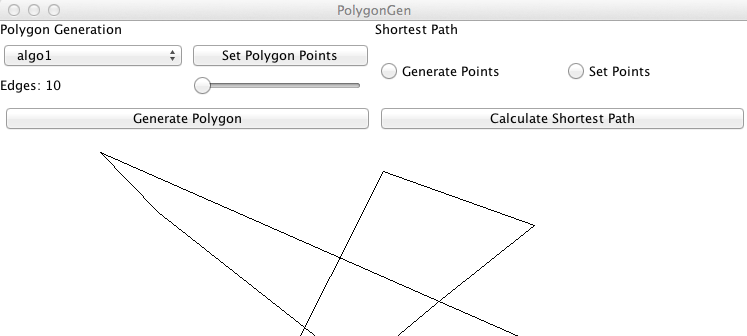
\includegraphics[width=1.00\textwidth]{PolygonGen.png}
\end{center}
\end{frame}

\end{document}

